% Options for packages loaded elsewhere
\PassOptionsToPackage{unicode}{hyperref}
\PassOptionsToPackage{hyphens}{url}
%
\documentclass[
]{article}
\usepackage{lmodern}
\usepackage{amssymb,amsmath}
\usepackage{ifxetex,ifluatex}
\ifnum 0\ifxetex 1\fi\ifluatex 1\fi=0 % if pdftex
  \usepackage[T1]{fontenc}
  \usepackage[utf8]{inputenc}
  \usepackage{textcomp} % provide euro and other symbols
\else % if luatex or xetex
  \usepackage{unicode-math}
  \defaultfontfeatures{Scale=MatchLowercase}
  \defaultfontfeatures[\rmfamily]{Ligatures=TeX,Scale=1}
\fi
% Use upquote if available, for straight quotes in verbatim environments
\IfFileExists{upquote.sty}{\usepackage{upquote}}{}
\IfFileExists{microtype.sty}{% use microtype if available
  \usepackage[]{microtype}
  \UseMicrotypeSet[protrusion]{basicmath} % disable protrusion for tt fonts
}{}
\makeatletter
\@ifundefined{KOMAClassName}{% if non-KOMA class
  \IfFileExists{parskip.sty}{%
    \usepackage{parskip}
  }{% else
    \setlength{\parindent}{0pt}
    \setlength{\parskip}{6pt plus 2pt minus 1pt}}
}{% if KOMA class
  \KOMAoptions{parskip=half}}
\makeatother
\usepackage{xcolor}
\IfFileExists{xurl.sty}{\usepackage{xurl}}{} % add URL line breaks if available
\IfFileExists{bookmark.sty}{\usepackage{bookmark}}{\usepackage{hyperref}}
\hypersetup{
  pdftitle={Parcial 1: Modelos lineales generalizados y no paramétricos},
  pdfauthor={Angie Rodríguez Duque},
  hidelinks,
  pdfcreator={LaTeX via pandoc}}
\urlstyle{same} % disable monospaced font for URLs
\usepackage[margin=1in]{geometry}
\usepackage{color}
\usepackage{fancyvrb}
\newcommand{\VerbBar}{|}
\newcommand{\VERB}{\Verb[commandchars=\\\{\}]}
\DefineVerbatimEnvironment{Highlighting}{Verbatim}{commandchars=\\\{\}}
% Add ',fontsize=\small' for more characters per line
\usepackage{framed}
\definecolor{shadecolor}{RGB}{248,248,248}
\newenvironment{Shaded}{\begin{snugshade}}{\end{snugshade}}
\newcommand{\AlertTok}[1]{\textcolor[rgb]{0.94,0.16,0.16}{#1}}
\newcommand{\AnnotationTok}[1]{\textcolor[rgb]{0.56,0.35,0.01}{\textbf{\textit{#1}}}}
\newcommand{\AttributeTok}[1]{\textcolor[rgb]{0.77,0.63,0.00}{#1}}
\newcommand{\BaseNTok}[1]{\textcolor[rgb]{0.00,0.00,0.81}{#1}}
\newcommand{\BuiltInTok}[1]{#1}
\newcommand{\CharTok}[1]{\textcolor[rgb]{0.31,0.60,0.02}{#1}}
\newcommand{\CommentTok}[1]{\textcolor[rgb]{0.56,0.35,0.01}{\textit{#1}}}
\newcommand{\CommentVarTok}[1]{\textcolor[rgb]{0.56,0.35,0.01}{\textbf{\textit{#1}}}}
\newcommand{\ConstantTok}[1]{\textcolor[rgb]{0.00,0.00,0.00}{#1}}
\newcommand{\ControlFlowTok}[1]{\textcolor[rgb]{0.13,0.29,0.53}{\textbf{#1}}}
\newcommand{\DataTypeTok}[1]{\textcolor[rgb]{0.13,0.29,0.53}{#1}}
\newcommand{\DecValTok}[1]{\textcolor[rgb]{0.00,0.00,0.81}{#1}}
\newcommand{\DocumentationTok}[1]{\textcolor[rgb]{0.56,0.35,0.01}{\textbf{\textit{#1}}}}
\newcommand{\ErrorTok}[1]{\textcolor[rgb]{0.64,0.00,0.00}{\textbf{#1}}}
\newcommand{\ExtensionTok}[1]{#1}
\newcommand{\FloatTok}[1]{\textcolor[rgb]{0.00,0.00,0.81}{#1}}
\newcommand{\FunctionTok}[1]{\textcolor[rgb]{0.00,0.00,0.00}{#1}}
\newcommand{\ImportTok}[1]{#1}
\newcommand{\InformationTok}[1]{\textcolor[rgb]{0.56,0.35,0.01}{\textbf{\textit{#1}}}}
\newcommand{\KeywordTok}[1]{\textcolor[rgb]{0.13,0.29,0.53}{\textbf{#1}}}
\newcommand{\NormalTok}[1]{#1}
\newcommand{\OperatorTok}[1]{\textcolor[rgb]{0.81,0.36,0.00}{\textbf{#1}}}
\newcommand{\OtherTok}[1]{\textcolor[rgb]{0.56,0.35,0.01}{#1}}
\newcommand{\PreprocessorTok}[1]{\textcolor[rgb]{0.56,0.35,0.01}{\textit{#1}}}
\newcommand{\RegionMarkerTok}[1]{#1}
\newcommand{\SpecialCharTok}[1]{\textcolor[rgb]{0.00,0.00,0.00}{#1}}
\newcommand{\SpecialStringTok}[1]{\textcolor[rgb]{0.31,0.60,0.02}{#1}}
\newcommand{\StringTok}[1]{\textcolor[rgb]{0.31,0.60,0.02}{#1}}
\newcommand{\VariableTok}[1]{\textcolor[rgb]{0.00,0.00,0.00}{#1}}
\newcommand{\VerbatimStringTok}[1]{\textcolor[rgb]{0.31,0.60,0.02}{#1}}
\newcommand{\WarningTok}[1]{\textcolor[rgb]{0.56,0.35,0.01}{\textbf{\textit{#1}}}}
\usepackage{graphicx,grffile}
\makeatletter
\def\maxwidth{\ifdim\Gin@nat@width>\linewidth\linewidth\else\Gin@nat@width\fi}
\def\maxheight{\ifdim\Gin@nat@height>\textheight\textheight\else\Gin@nat@height\fi}
\makeatother
% Scale images if necessary, so that they will not overflow the page
% margins by default, and it is still possible to overwrite the defaults
% using explicit options in \includegraphics[width, height, ...]{}
\setkeys{Gin}{width=\maxwidth,height=\maxheight,keepaspectratio}
% Set default figure placement to htbp
\makeatletter
\def\fps@figure{htbp}
\makeatother
\setlength{\emergencystretch}{3em} % prevent overfull lines
\providecommand{\tightlist}{%
  \setlength{\itemsep}{0pt}\setlength{\parskip}{0pt}}
\setcounter{secnumdepth}{-\maxdimen} % remove section numbering

\title{Parcial 1: Modelos lineales generalizados y no paramétricos}
\author{Angie Rodríguez Duque}
\date{Octubre 23 de 2020}

\begin{document}
\maketitle

\hypertarget{introducciuxf3n}{%
\section{Introducción}\label{introducciuxf3n}}

El presente trabajo tiene como finalidad ajustar un Modelo Logístico,
para un conjunto de datos de vino tinto que consta de 1599 observaciones
y 12 variables, 11 de las cuales son sustancias químicas.

\begin{Shaded}
\begin{Highlighting}[]
\KeywordTok{dim}\NormalTok{(Datos)}
\end{Highlighting}
\end{Shaded}

\begin{verbatim}
## [1] 1599   12
\end{verbatim}

Las variables son:

\begin{enumerate}
\def\labelenumi{\arabic{enumi}.}
\item
  \textbf{Acidez fija:} La mayoría de los ácidos implicados en el vino
  son fijos o no volátiles (no se evaporan fácilmente).
\item
  \textbf{Acidez volátil:} La cantidad de ácido acético en el vino, que
  en niveles demasiado altos puede provocar un sabor desagradable a
  vinagre.
\item
  \textbf{Ácido cítrico:} Encontrado en pequeñas cantidades, el ácido
  cítrico puede agregar ``frescura'' y sabor a los vinos.
\item
  \textbf{Azúcar residual:} Es la cantidad de azúcar que queda después
  de que se detiene la fermentación, es raro encontrar vinos con menos
  de 1 gramo / litro y los vinos con más de 45 gramos / litro se
  consideran dulces.
\item
  \textbf{Cloruros:} Es la cantidad de sal del vino.
\item
  \textbf{Dióxido de azufre libre:} La forma libre de \(SO_{2}\) existe
  en equilibrio entre el \(SO_{2}\) molecular (como gas disuelto) y el
  ion bisulfito; Previene el crecimiento microbiano y la oxidación del
  vino.
\item
  \textbf{Dióxido de azufre total:} Es la cantidad de formas libres y
  unidas de \(SO_{2}\); en concentraciones bajas, el \(SO_{2}\) es
  mayormente indetectable en el vino, pero en concentraciones de
  \(SO_{2}\) libre superiores a 50 ppm, el \(SO_{2}\) se hace evidente
  en la nariz y el sabor del vino.
\item
  \textbf{Densidad:} La densidad es cercana a la del agua dependiendo
  del porcentaje de alcohol y contenido de azúcar.
\item
  \textbf{pH:} Describe qué tan ácido o básico es un vino en una escala
  de 0 (muy ácido) a 14 (muy básico); la mayoría de los vinos están
  entre 3-4 en la escala de pH.
\item
  \textbf{Sulfatos:} Aditivo del vino que puede contribuir a los niveles
  de dióxido de azufre \((SO_{2})\), que actúa como antimicrobiano y
  antioxidante.
\item
  \textbf{Alcohol:} El porcentaje de contenido de alcohol del vino.
\item
  \textbf{Calidad:} Variable de respuesta (basada en datos sensoriales,
  puntuación entre 0 y 10).
\end{enumerate}

\hypertarget{estaduxedsticas-descriptivas}{%
\subsubsection{Estadísticas
descriptivas}\label{estaduxedsticas-descriptivas}}

\begin{Shaded}
\begin{Highlighting}[]
\KeywordTok{summary}\NormalTok{(Datos)}
\end{Highlighting}
\end{Shaded}

\begin{verbatim}
##  fixed.acidity   volatile.acidity  citric.acid    residual.sugar  
##  Min.   : 4.60   Min.   :0.1200   Min.   :0.000   Min.   : 0.900  
##  1st Qu.: 7.10   1st Qu.:0.3900   1st Qu.:0.090   1st Qu.: 1.900  
##  Median : 7.90   Median :0.5200   Median :0.260   Median : 2.200  
##  Mean   : 8.32   Mean   :0.5278   Mean   :0.271   Mean   : 2.539  
##  3rd Qu.: 9.20   3rd Qu.:0.6400   3rd Qu.:0.420   3rd Qu.: 2.600  
##  Max.   :15.90   Max.   :1.5800   Max.   :1.000   Max.   :15.500  
##    chlorides       free.sulfur.dioxide total.sulfur.dioxide    density      
##  Min.   :0.01200   Min.   : 1.00       Min.   :  6.00       Min.   :0.9901  
##  1st Qu.:0.07000   1st Qu.: 7.00       1st Qu.: 22.00       1st Qu.:0.9956  
##  Median :0.07900   Median :14.00       Median : 38.00       Median :0.9968  
##  Mean   :0.08747   Mean   :15.87       Mean   : 46.47       Mean   :0.9967  
##  3rd Qu.:0.09000   3rd Qu.:21.00       3rd Qu.: 62.00       3rd Qu.:0.9978  
##  Max.   :0.61100   Max.   :72.00       Max.   :289.00       Max.   :1.0037  
##        pH          sulphates         alcohol         quality     
##  Min.   :2.740   Min.   :0.3300   Min.   : 8.40   Min.   :3.000  
##  1st Qu.:3.210   1st Qu.:0.5500   1st Qu.: 9.50   1st Qu.:5.000  
##  Median :3.310   Median :0.6200   Median :10.20   Median :6.000  
##  Mean   :3.311   Mean   :0.6581   Mean   :10.42   Mean   :5.636  
##  3rd Qu.:3.400   3rd Qu.:0.7300   3rd Qu.:11.10   3rd Qu.:6.000  
##  Max.   :4.010   Max.   :2.0000   Max.   :14.90   Max.   :8.000
\end{verbatim}

\begin{figure}
\centering
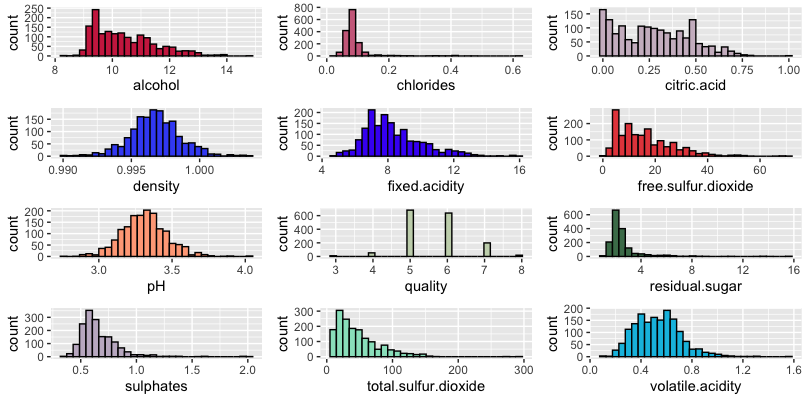
\includegraphics[width=6.77083in,height=\textheight]{G1.png}
\caption{Distribución de las variables}
\end{figure}

\hypertarget{observaciones}{%
\subsubsection{Observaciones}\label{observaciones}}

\begin{itemize}
\item
  Algunas de las variables tienen distribuciones normales (densidad,
  acidez fija, pH, acidez volátil).
\item
  Algunas variables están un poco sesgadas hacia el extremo inferior de
  los valores (cloruros, ácido cítrico, azúcar residual, dióxido de
  azufre total).
\item
  La variable calidad tiene solo 6 valores discretos.
\end{itemize}

\hypertarget{correlaciuxf3n}{%
\subsubsection{Correlación}\label{correlaciuxf3n}}

\begin{Shaded}
\begin{Highlighting}[]
\KeywordTok{corrplot}\NormalTok{(}\KeywordTok{cor}\NormalTok{(Datos), }\DataTypeTok{method=}\StringTok{"square"}\NormalTok{, }\DataTypeTok{type=}\StringTok{"upper"}\NormalTok{, }\DataTypeTok{order=}\StringTok{"hclust"}\NormalTok{, }\DataTypeTok{tl.col=}\StringTok{"black"}\NormalTok{)}
\end{Highlighting}
\end{Shaded}

\begin{center}\includegraphics{Parcial2_AngieRodriguez_files/figure-latex/unnamed-chunk-5-1} \end{center}

\begin{itemize}
\item
  La densidad tiene una correlación muy fuerte con la acidez fija.
\item
  Las variables más fuertemente correlacionadas con la calidad son la
  acidez volátil y el alcohol.
\item
  El alcohol tiene una correlación negativa con la densidad. Esto es
  evidente por el hecho de que la densidad del agua es mayor que la
  densidad del alcohol.
\item
  Es posible observar que las variables pH y acidez fija presentan una
  correlación negativamente fuerte, lo cual nos indica que a mayor pH
  menor será la acidez, y viceversa, a menor pH mayor acidez. Lo cual se
  ve reflejado en la calidad final del vino.
\end{itemize}

\hypertarget{muestra}{%
\section{Muestra}\label{muestra}}

Se elige una muestra de mil doscientos \((1200)\) vinos de esta base de
datos y trabaje, tal como sigue:

\begin{Shaded}
\begin{Highlighting}[]
\CommentTok{#Tamaño de la muestra}
\NormalTok{n <-}\StringTok{ }\DecValTok{1200}
\end{Highlighting}
\end{Shaded}

\hypertarget{variable-indicadora-alcoholab}{%
\subsubsection{Variable indicadora:
alcoholAB}\label{variable-indicadora-alcoholab}}

Se convierte la variable ``alcohol'' en una variable indicadora con dos
niveles: ``bajo'' y ``alto'', esta nueva variable se denomina:
``alcoholAB''. Para dicha transformación se realiza el siguiente
procedimiento:

\hypertarget{variables-dicotomica-calidadab}{%
\subsection{Variables dicotomica:
calidadAB}\label{variables-dicotomica-calidadab}}

Se convierte la variable calidad (quality) en una variable dicotómica y
se denomina ``calidadAB''. Se forma un grupo con los vinos que tienen
calidades 7 y 8 y otro con los demás vinos.

\begin{Shaded}
\begin{Highlighting}[]
\CommentTok{# Variable indicadora alcoholAB}
\NormalTok{alcoholAB <-}\StringTok{ }\KeywordTok{vector}\NormalTok{() }
\NormalTok{alcoholAB[muestra}\OperatorTok{$}\NormalTok{alcohol }\OperatorTok{<}\StringTok{ }\DecValTok{12}\NormalTok{] <-}\StringTok{ "Bajo"}
\NormalTok{alcoholAB[muestra}\OperatorTok{$}\NormalTok{alcohol }\OperatorTok{>=}\StringTok{ }\DecValTok{12}\NormalTok{] <-}\StringTok{ "Alto"}
\NormalTok{alcoholAB <-}\StringTok{ }\KeywordTok{as.factor}\NormalTok{(alcoholAB)}
\KeywordTok{table}\NormalTok{(alcoholAB)}
\end{Highlighting}
\end{Shaded}

\begin{verbatim}
## alcoholAB
## Alto Bajo 
##  124 1076
\end{verbatim}

\begin{Shaded}
\begin{Highlighting}[]
\CommentTok{# Variable indicadora quality}
\NormalTok{calidadAB <-}\StringTok{ }\KeywordTok{vector}\NormalTok{()}
\NormalTok{calidadAB[muestra}\OperatorTok{$}\NormalTok{quality }\OperatorTok{<=}\StringTok{ }\DecValTok{6}\NormalTok{] <-}\StringTok{ "0"}
\NormalTok{calidadAB[muestra}\OperatorTok{$}\NormalTok{quality }\OperatorTok{>}\StringTok{ }\DecValTok{6}\NormalTok{] <-}\StringTok{ "1"}
\NormalTok{calidadAB <-}\StringTok{ }\KeywordTok{as.factor}\NormalTok{(calidadAB)}
\KeywordTok{table}\NormalTok{(calidadAB)}
\end{Highlighting}
\end{Shaded}

\begin{verbatim}
## calidadAB
##    0    1 
## 1024  176
\end{verbatim}

\hypertarget{modelo-loguxedstico-con-variable-indicadora}{%
\section{Modelo logístico con variable
indicadora}\label{modelo-loguxedstico-con-variable-indicadora}}

Para ajustar este modelo se hace uso de la función glm() para modelos
lineales generalizados, una clase de modelos en los que se incluye el
modelo logístico. En nuestro caso, como la variable de respuesta
``calidadAB''es una variable dicotómica especificamos el argumento
family = binomial.

Ajuste un modelo lineal generalizado usando como respuesta la variable
calidadAB y como variables de predicción las variables ``acidez fja''
(fixed acidity) y ``alcoholAB''.

\[calidadAB= Acidez fija+AlcoholAB +Acidez fija*AlcoholAB\]

\begin{Shaded}
\begin{Highlighting}[]
\NormalTok{modelo.logit <-}\StringTok{ }\KeywordTok{glm}\NormalTok{(calidadAB }\OperatorTok{~}\StringTok{ }\NormalTok{fixed.acidity }\OperatorTok{+}\StringTok{ }\NormalTok{alcoholAB, }\DataTypeTok{data =}\NormalTok{ muestra, }\DataTypeTok{family =} \StringTok{"binomial"}\NormalTok{)}
\end{Highlighting}
\end{Shaded}

\begin{Shaded}
\begin{Highlighting}[]
\KeywordTok{summary}\NormalTok{(modelo.logit)}
\end{Highlighting}
\end{Shaded}

\begin{verbatim}
## 
## Call:
## glm(formula = calidadAB ~ fixed.acidity + alcoholAB, family = "binomial", 
##     data = muestra)
## 
## Deviance Residuals: 
##     Min       1Q   Median       3Q      Max  
## -1.7320  -0.5047  -0.4466  -0.4181   2.2768  
## 
## Coefficients:
##               Estimate Std. Error z value Pr(>|z|)    
## (Intercept)   -1.49667    0.40226  -3.721 0.000199 ***
## fixed.acidity  0.17258    0.04525   3.814 0.000137 ***
## alcoholABBajo -2.07012    0.21092  -9.815  < 2e-16 ***
## ---
## Signif. codes:  0 '***' 0.001 '**' 0.01 '*' 0.05 '.' 0.1 ' ' 1
## 
## (Dispersion parameter for binomial family taken to be 1)
## 
##     Null deviance: 1000.52  on 1199  degrees of freedom
## Residual deviance:  901.35  on 1197  degrees of freedom
## AIC: 907.35
## 
## Number of Fisher Scoring iterations: 4
\end{verbatim}

De acuerdo a los resultados obtenidos y teniendo en cuenta que la
interpretación de los p-valores es similar a la del modelo lineal.
Podemos ver que las variables statusquo y sexo son altamente
significativas (\textless2e-16 y 0.000277).

En cuanto a los coeficientes del modelo logit, estos se interpretan como
el logaritmo del odds ratio. De esta manera, si nos fijamos en el
coeficiente de la variable statusquo (3.2085), está positivamente
relacionada con el logaritmo del odds ratio de la intención de voto, el
cual aumentaría 3.2085 unidades por cada unidad que aumenta la
puntuación en el statusquo.

\hypertarget{bibliografuxeda}{%
\section{Bibliografía}\label{bibliografuxeda}}

\begin{itemize}
\tightlist
\item
  Fox, J. (2015),Applied regression analysis and generalized linear
  models, SagePublications.
\item
  Dobson, A. J., \& Barnett, A. G. (2018). An introduction to
  generalized linear models. CRC press.
\end{itemize}

\end{document}
